\begin{frame}{Supervised Fine-Tuning (SFT)}
  \begin{center}
    \Large
    Supervised Fine-Tuning (SFT)
  \end{center}
\end{frame}


\begin{frame}{What is Supervised Fine-Tuning (SFT)?}
  \begin{figure}
    \centering
    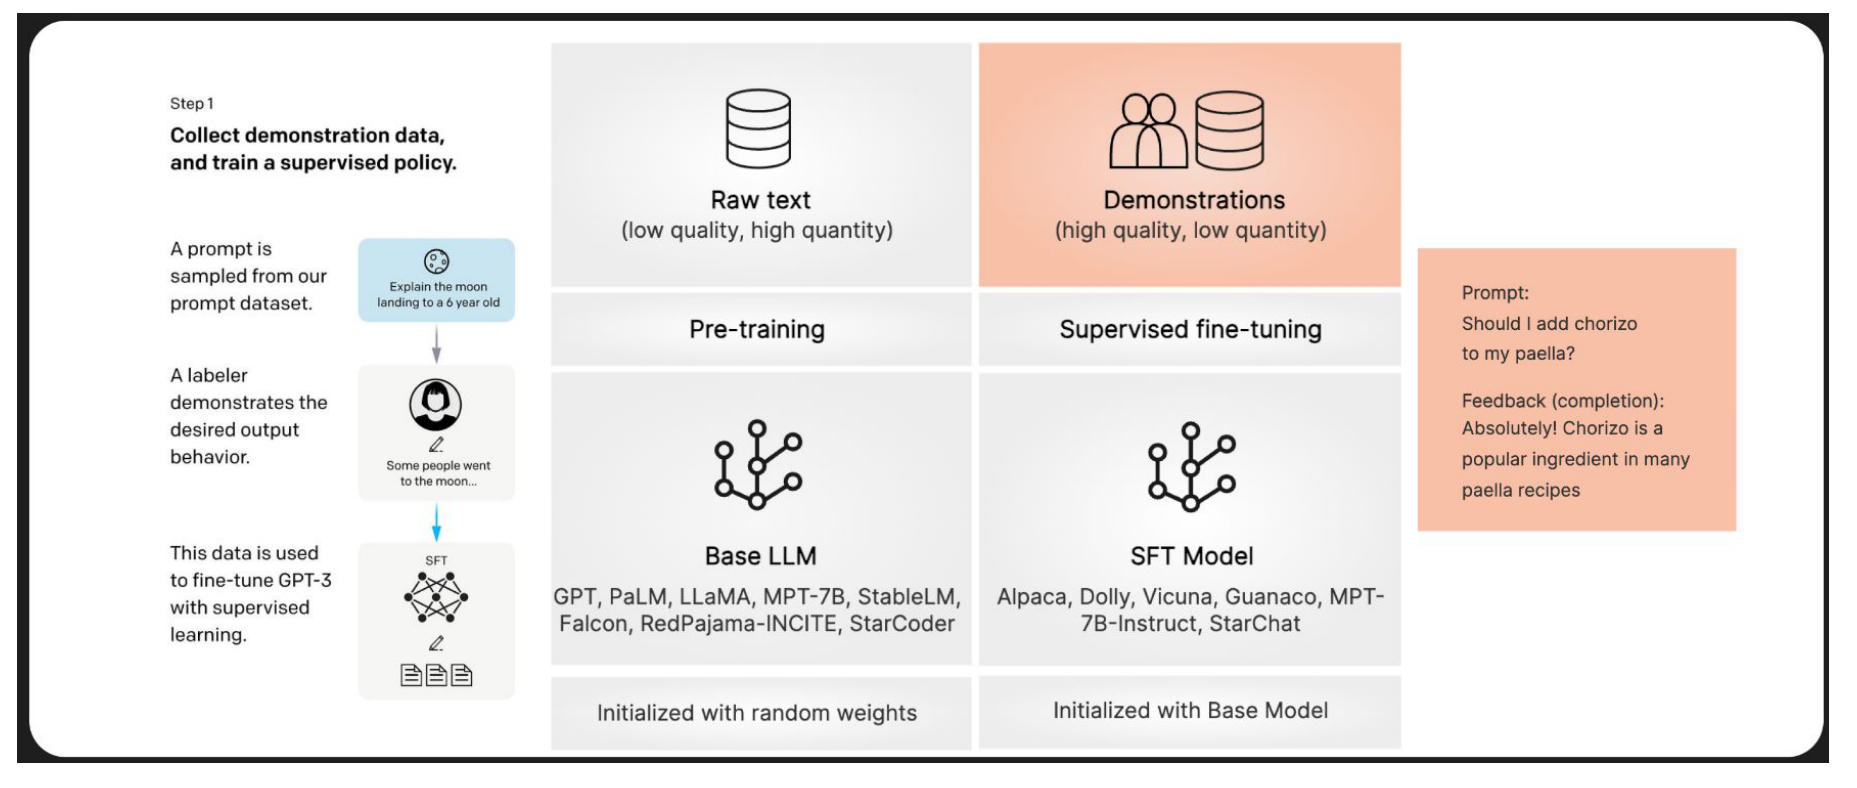
\includegraphics[width=0.60\paperwidth,height=0.58\paperheight,keepaspectratio]{images/llm-rlhf/finetune_sft_pretraining_pipeline.png}
    \caption*{\scriptsize Source: Argilla, ``Collecting RLHF data'' (docs.argilla.io); left panel from Ouyang et al., 2022.}
  \end{figure}
\end{frame}

\begin{frame}{Supervised Fine-Tuning For Gemini LLM}
  \begin{figure}
    \centering
    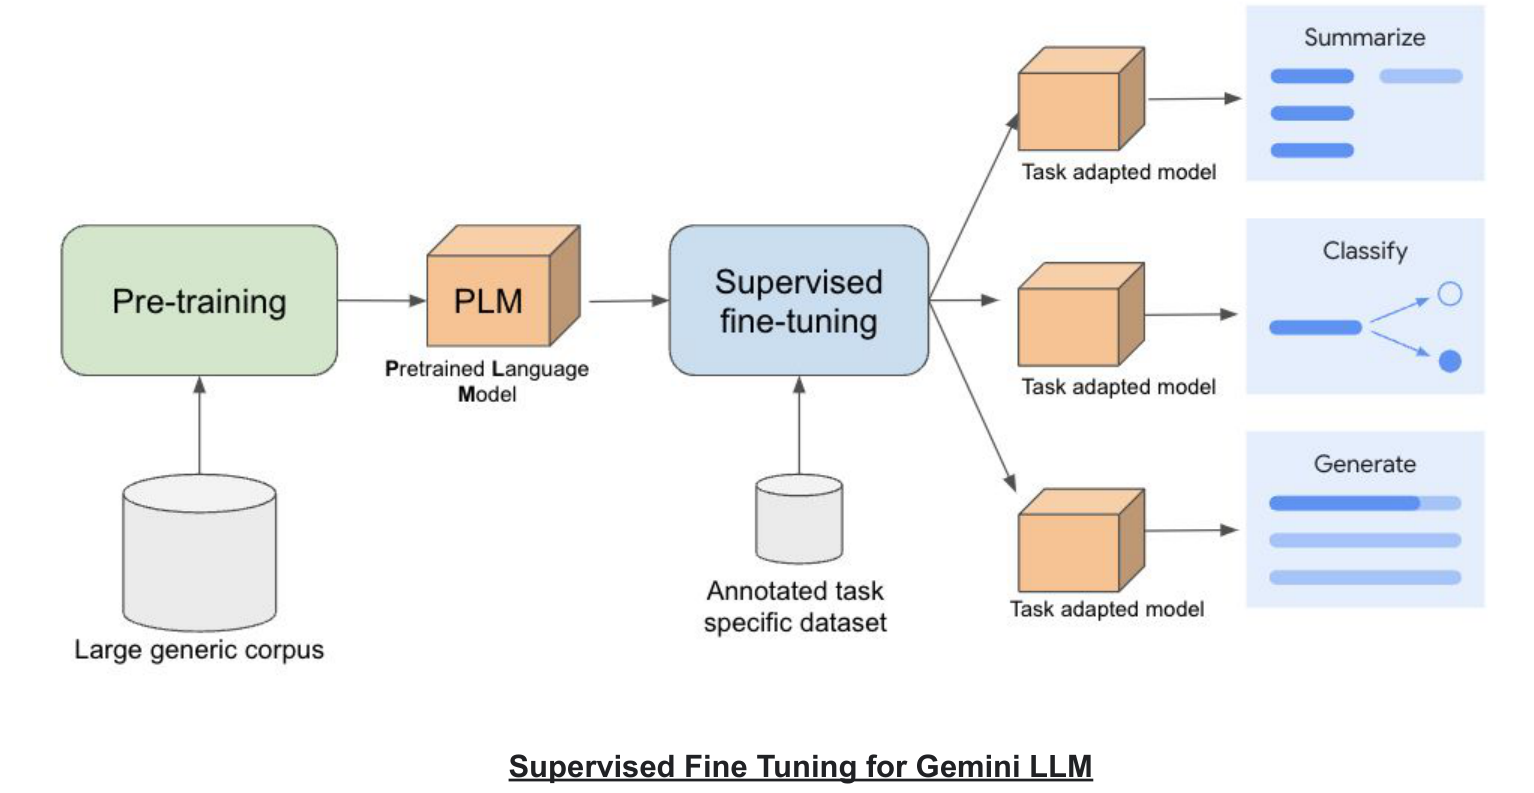
\includegraphics[width=0.60\paperwidth,height=0.58\paperheight,keepaspectratio]{images/llm-rlhf/finetune_sft_task_adaptation.png}
    \caption*{\scriptsize Source: E.~Huizenga \& M.~Hu, ``When to use supervised fine-tuning for Gemini,'' Google Cloud Blog, 2024.}
  \end{figure}
\end{frame}

\begin{frame}{Datasets for Supervised Fine-Tuning (SFT)}
  \begin{itemize}
    \item \textbf{Instructional datasets:}
    \begin{itemize}
      \item \textbf{OpenAI:} InstructGPT, roughly 13k labeler-written demonstrations (never released publicly)
      \item \textbf{Stanford Alpaca:} 52k instructions generated with OpenAI's \texttt{text-davinci-003} using the Self-Instruct recipe
      \item \textbf{Others:} databricks-dolly-15k, ShareGPT, OASST1, UltraChat
    \end{itemize}
    \item[\textcolor{red}{$\blacktriangleright$}] Note where each one came from: Dolly and OASST1 are human-written, Alpaca and UltraChat are model-generated, ShareGPT is scraped conversations.
    \item[\textcolor{red}{$\blacktriangleright$}] \textbf{Note:} Quality of supervision greatly affects model behavior.
  \end{itemize}
\end{frame}

\begin{frame}{Domain-Specific SFT: Finance}
  \begin{itemize}\itemsep0.4em
    \item[\textcolor{red}{$\blacktriangleright$}] General instruction data teaches broad helpfulness; \textbf{domain-specific SFT} adapts a model to a vertical using labeled in-domain data.
    \item[\textcolor{red}{$\blacktriangleright$}] \textbf{Finance datasets:}
      \begin{itemize}
        \item \textbf{FiQA} (WWW'18 challenge): aspect-based financial sentiment and opinion-based question answering.
        \item \textbf{Financial PhraseBank} (Malo et al., 2014): 4{,}845 financial-news sentences labeled positive / negative / neutral from an investor's point of view by annotators with a finance background.
        \item \textbf{SEC filings (10-K):} long regulatory filings used to tune models that read earnings reports and risk statements.
      \end{itemize}
  \end{itemize}
\end{frame}

\begin{frame}[t]{Two Routes to a Domain Model}
  \begin{itemize}\itemsep0.5em
    \item[\textcolor{red}{$\blacktriangleright$}] \textbf{Fine-tune an existing model.} \textbf{FinBERT} (Araci, 2019) is this recipe exactly: BERT further trained on a Reuters financial corpus, then fine-tuned on Financial PhraseBank. It reaches 0.86 accuracy where a same-size general model reaches 0.83.
    \item[\textcolor{red}{$\blacktriangleright$}] \textbf{Pre-train from scratch on a mixed corpus.} \textbf{BloombergGPT} used 363B financial and 345B general tokens. Far more expensive, and worth it only with proprietary data at that scale.
    \item[\textcolor{red}{$\blacktriangleright$}] For almost everyone the first route is the right one, and the same recipe applies to law, medicine, and code: a modest, high-quality in-domain set often beats a much larger generic one.
  \end{itemize}
\end{frame}

\begin{frame}{Limitations of Supervised Fine-Tuning (SFT)}
  \begin{itemize}
    \item[\textcolor{red}{$\blacktriangleright$}] Cannot capture nuanced human preferences or values.
    \item[\textcolor{red}{$\blacktriangleright$}] May reinforce existing biases or hallucinations present in the data.
    \item[\textcolor{red}{$\blacktriangleright$}] Risk of overfitting, especially on synthetic or noisy datasets.
    \item[\textcolor{red}{$\blacktriangleright$}] Often leads to safe but bland and generic responses.
  \end{itemize}
\end{frame}
